\documentclass[oneside,spanish]{amsart}
\usepackage[T1]{fontenc}
\usepackage[utf8]{inputenc}
\usepackage[a4paper]{geometry}
\geometry{verbose,tmargin=2cm,bmargin=2cm,lmargin=3cm,rmargin=2.5cm}
\usepackage{amsthm}
\usepackage{enumitem}
\usepackage{graphicx}
\usepackage{tikz}
\usepackage{float}
\usepackage{apacite}
\usepackage{hyperref}
\usepackage{url}
\usepackage{fancyhdr}

\makeatletter
%Numeraci�n
\numberwithin{equation}{section}
\numberwithin{figure}{section}
\newlength{\lyxlabelwidth}      % Longitud auxiliar

\makeatother

\usepackage{babel}
\addto\shorthandsspanish{\spanishdeactivate{~<>}}

\pagestyle{fancy}
\fancyhf{}


\begin{document}
\title{El desarrollo del pensamiento proporcional en la primaria y el ciclo básico del nivel secundario haciendo uso de los registros semióticos de representación y las TIC}
\maketitle
\noindent \begin{flushright}
\textsl{\small{}Taller}{\small{} }{\small\par}
\par\end{flushright}

\section{Introducción}

\subsection{Importancia del Taller}

Es importante que los estudiantes desarrollen el pensamiento proporcional para que logren la comprensión conceptual de la proporcionalidad y así  puedan desempeñarse con fluidez en su vida cotidiana. Pero también para que puedan  construir conceptos más complejos en niveles educativos superiores , como por ejemplo  las variaciones, la función lineal, las razones de cambios, las derivadas. Por eso es necesario generar un espacio de reflexión sobre la enseñanza y aprendizaje de la proporcionalidad, que permita poner en relevancia los diferentes significados de la proporcionalidad haciendo uso de los distintos registros semióticos e incluyendo las TIC. 

\subsection{Fundamentos}

En general los estudiantes del nivel secundario y los ingresantes al nivel superior  muestran que tienen dificultades al resolver situaciones vinculadas a la proporcionalidad.  Para lograr que haya una buena comprensión conceptual de la proporcionalidad es preciso que el estudiante desarrolle el pensamiento proporcional, tal como lo señala Piaget (1978) al expresar que para que el estudiante de nivel básico le de sentido y significado a la proporcionalidad es fundamental desarrollar su pensamiento proporcional cualitativo y cuantitativo. Van Dooren, De Bock, Janssens y Verschaffel (2005) consideran que además el estudiante debe tener la habilidad de discriminar entre situaciones proporcionales y no proporcionales como un dominio del conocimiento del razonamiento proporcional.

En la enseñanza de la proporcionalidad es necesario considerar los diferentes significados. Al respecto  Godino, Beltrán-Pellicer, Burgos y Giacomone (2017) expresan que los  significados de la proporcionalidad se pueden clasificar según criterios, en particular, el contexto o campo de aplicación y el nivel de algebrización de las prácticas matemáticas realizadas. Algunos contextos de aplicación de las nociones de razón y proporción (vida cotidiana, científicotécnico, artístico, geométrico, probabilístico, estadístico, etc.) deben ser incluídos  en las prácticas de resolución de los problemas adecuados al nivel de escolaridad. Los mismos autores también  distinguen tres tipos de significados de la proporcionalidad: aritmético, proto-algebraico y algebraico-funcional, que deben ser considerados en la enseñanza aprendizaje de este concepto.

En la actualidad el desafío pedagógico en matemática, en la escuela primaria y secundaria, consiste en lograr un aprendizaje significativo en los estudiantes, a partir de situaciones de aprendizaje que permitan desarrollar sus capacidades. En el Marco Nacional para la mejora  del aprendizaje en Matemática  [Ministerio de Educación, Cultura, Ciencia y Tecnología, 2019] se plantea mejorar el aprendizaje en matemática y desarrollar el potencial del pensamiento lógico matemático, siendo una posibilidad  la incorporación de herramientas tecnológicas en la resolución de problemas. No menos importante resulta, según Duval (2004), la interacción entre los distintos tipos de registros: natural, numérico, gráfico, geométrico y algebraico para propiciar aprendizajes significativos de los conceptos y  como forma de ligar el tratamiento de la información con la experiencia de los estudiantes. Es necesario que los estudiantes aprendan a usar las Tecnologías de la Información y Comunicación y a interactuar con ellas, de allí que los docentes deban incluir  estas nuevas tecnologías en las propuestas educativas. Particularmente el Software dinámico Geogebra permite la coordinación de los diferentes registros y de esta manera se convierte en una potente herramienta para propiciar la significación de conceptos, en este caso de la proporcionalidad que funciona en diferentes registros.

\section{Contenidos}

Situaciones aditivas y proporcionales. Errores frecuentes de los estudiantes. Pensamiento Proporcional: Caracterización. Pensamiento proporcional  cualitativo y cuantitativo. Significado aritmético, proto-algebraico y algebraico-funcional de la proporcionalidad. Registros semióticos de representación. Uso de TIC.

\section{Requisitos Previos}

Ser docente de matemática de 6to o 7mo año del Nivel Primario o docente de matemática del Nivel Secundario. También podría ser un estudiante avanzado del Profesorado de Matemática.

Es necesario que tenga ideas básicas de Proporcionalidad y que tenga conocimiento de las  herramientas básicas de Geogebra.


\section{Objetivos}
\begin{itemize}[itemsep=10pt]
    \item Reflexionar sobre los errores frecuentes de los estudiantes cuando resuelven situaciones de proporcionalidad.
    \item Valorar la necesidad de promover el desarrollo del pensamiento proporcional en los estudiantes.
    \item Reconocer los diferentes significados de la proporcionalidad.
    \item Propiciar el uso de registros semióticos y la inclusión de recursos informáticos para potenciar las producciones matemáticas de los estudiantes.
    \item Repensar la articulación entre el Nivel Primario y Secundario en torno a   la enseñanza de la proporcionalidad.
\end{itemize}
\section{Actividades}

\subsection{Actividades Previas}

\begin{description}[itemsep=10pt]
    \item[Contenidos] Situaciones aditivas y de proporcionalidad. Errores frecuentes de los estudiantes cuando resuelven situaciones de proporcionalidad.
    
    \item[Actividad 1] Los asistentes deberán resolver problemas y luego clasificarlos en aditivos o de proporcionalidad.

    Además, deberán proponer una resolución correcta y otra incorrecta que podrían realizar los estudiantes para alguno de los problemas.
    \begin{enumerate}[label=\alph*), itemsep=10pt]
      \item Una máquina llena 26 cajones de pescado por hora siempre a la misma velocidad.
      
      ¿Cuánto tardará para llenar 78 cajones? ¿Y 156? Si la máquina estuvo trabajando 5 horas, ¿Cuántos cajones se llenaron? Expliquen cómo llegaron a su respuesta.
      \item Pedro y Tomás están cargando cajas en un camión. Empezaron al mismo tiempo, pero Tomás es más rápido. Cuando Pedro ha cargado 5 cajas, Tomás ha cargado 10 cajas. Si Pedro ha cargado 28 cajas, ¿Cuántas cajas ha cargado Tomás?
      \item Pedro y Tomás están cargando cajas en un camión. Cargan a la misma velocidad, pero Pedro empezó más tarde. Cuando Pedro ha cargado 4 cajas, Tomás ha cargado 10 cajas. Si   Pedro ha cargado 20   cajas, ¿Cuántas cajas ha cargado Tomás?
      \item El profesor le dijo a Nicolas que hiciese más fotocopias. Nicolas cometió un error y apretó el botón que reduce el tamaño de cada copia a  $\frac{3}{4}$. ¿Cuánto debe aumentar Nicolás el tamaño de las copias reducidas para corregir el tamaño original?
      \item Las empresas A y B fabrican tornillos a la misma velocidad, pero la empresa B ha empezado antes. Cuando la empresa A ha fabricado 40 cajas, la empresa B ha fabricado 120 cajas. Si la empresa A ha fabricado 120 cajas. ¿Cuántas cajas tendrá fabricada la empresa B?
    \end{enumerate}
    
    \item[Actividad 2] Analizarán un registro de un fragmento extraído de un artículo de Mendoza y Block (2013) donde un estudiante explica cómo resolvió una situación de proporcionalidad vinculada a porcentaje y responderán un cuestionario sobre el mismo.
\end{description}

\subsection{Primera hora y media presenciales\label{subsec:Primera-hora-y-media-sinc}}

\begin{description}[itemsep=10pt]
    \item[Contenidos] Errores frecuentes de los estudiantes cuando resuelven situaciones de proporcionalidad. Pensamiento Proporcional: caracterización. Pensamiento proporcional cualitativo y cuantitativo.

    Se recuperarán las producciones de la actividad previa y se caracterizarán los errores frecuentes.
    
    A través de un power point se definirá y caracterizará el pensamiento proporcional.

    En grupo se resolverán y analizarán actividades destinadas a los estudiantes de primaria. Un grupo resolverá una actividad con dos tareas  donde se utiliza el pensamiento proporcional cualitativo y el otro grupo una  actividad con dos tareas donde se utiliza el pensamiento proporcional cuantitativo.

    Ejemplo de una de las tareas de las actividades, propuesta por Ruiz, Elena, \& Valdemoros, Marta. (2006)

    El dibujo que está abajo es la casa de Antonio. El sacó una copia fotostática en reducción. De los dibujos que están más abajo marca la letra que corresponda a la reducción que obtuvo.

    \begin{figure}[h]
        \centering
        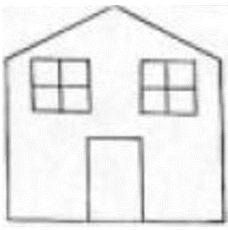
\includegraphics{imagenes/casa1.png}
        \label{fig:casa1}
    \end{figure}
    
    \begin{figure}[h]
        \centering
        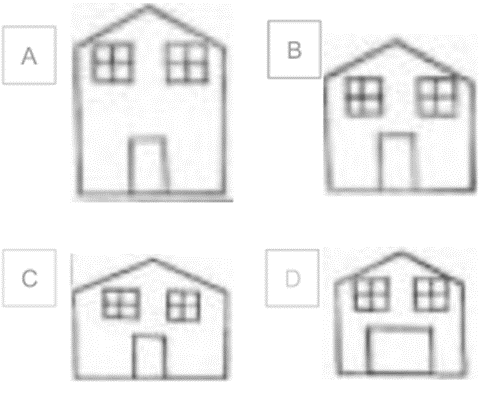
\includegraphics{imagenes/casa2.png}
        \label{fig:casa2}
    \end{figure}

    Escribe paso a paso que hiciste para resolverlo
    
    Se realizará una puesta común eligiendo los representantes de algunos grupos para la socialización.
    
    Los talleristas sintetizarán las producciones y señalarán la diferencia entre pensamiento proporcional cualitativo y cuantitativo y las actividades que les corresponden. Además, se mostrará una posible secuencia de tipo de pensamiento y actividades para ir articulando primaria con nivel secundario.


\end{description}

\subsection{Primeras dos horas Entre Clases\label{subsec:Primeras-dos-EC}}

\begin{description}[itemsep=10pt]
    \item[Actividad 1] Se les proporcionará el artículo “Significados pragmáticos y configuraciones ontosemióticas en el estudio de la proporcionalidad” de Godino et al (2017) donde se clasifican los significados de proporcionalidad.
    \item[Actividad 2] Deberán analizar actividades reconociendo el significado de proporcionalidad que enfatiza, según el texto de Godino y los contenidos matemáticos que subyacen.  Las actividades propuestas están destinadas a nivel primario y secundario. Además, deberán resolver una de las actividades que analizan.

    Ejemplo de una actividad que analizarán: (la siguiente actividad fue extraída de Atela, Fernández y Vila (2019))

    \item[Problema 1] El siguiente dibujo es un cuadrado  
    
\begin{tikzpicture}
      \draw (0,0) rectangle (1,1);
    \end{tikzpicture}

    \begin{enumerate}[label=\alph*), itemsep=10pt]
        \item Completa en cada caso el dato faltante:
            \begin{table}[h]
                \centering
                \begin{tabular}{|l|c|c|c|c|c|c|c|}\hline
                    Longitud del lado del cuadrado(cm) & 0 & 2 & 4 & 7 &  & 12 & 15 \\\hline
                    Perímetro del cuadrado(cm) &  & 8 &  &  & 40 &  &  \\ \hline
                \end{tabular}
                \label{tab:tabla-longitud-perimetro}
            \end{table}
        \item Si se duplica un par de lados, se obtiene un rectángulo. ¿El perímetro de la nueva figura se duplica? Justifiquen.
        \item Si se duplican los lados del cuadrado original, se obtiene otro cuadrado. ¿El cuadrado de la nueva figura se duplica? Justifiquen.
        \item Si se triplican los lados del cuadrado original, se obtiene otro cuadrado. ¿El perímetro de la nueva figura se triplica? Justifiquen.
        \item A partir de lo analizado, ¿En qué casos el perímetro es directamente proporcional a la longitud del lado?

    \end{enumerate}

     
\end{description}

\subsection{Segunda hora y media presencial}

\begin{description}[itemsep=10pt]
    \item[Contenidos] Significados de la proporcionalidad. Registros semióticos. 

    Se recuperará la resolución de la actividad entre clases solicitando a dos asistentes  que comenten sus resoluciones. Se realizará una síntesis sobre los significados de la proporcionalidad propuestos por Godino.
    
    A través de un power point se desarrollarán  los registros de representación Semiótica  de Duval (2004 ). 
    
    Se hará un breve repaso del uso de herramientas de Geogebra.
    
    En grupos se resolverá  una actividad para primaria con Geogebra. Además se  deberá identificar tipo de pensamiento, contenidos , significado y registros.\\

    Ahora analicen el archivo de Geogebra “problema 1” y sigan las instrucciones:(Actividad propuesta por Atela, Fernandez y Vila (2019))\\

    \begin{enumerate}[label=\alph*), itemsep=10pt]
        \item Muevan el punto a del deslizador, ¿Qué observan?, ¿Qué se modifica y qué se mantiene constante?, ¿Por qué creen que ocurre esto?
        \item ¿Qué significado tiene el valor de a? 
        \item ¿Qué sucede cuando a=0? ¿Coincide con el valor de la tabla que completaron en el problema 1 a)?
        \item Ahora muevan el punto A, ¿Qué se modifica y qué se mantiene constante? ¿Por qué consideran que ocurre esto?
        \item Ahora muevan el punto B, ¿Qué se modifica y qué se mantiene constante? ¿Por qué consideran que ocurre esto?
        \item Utilizando la Vista Algebraica y/o la vista gráfica completen la tabla:

            \begin{table}[h]
                \centering
                \begin{tabular}{|l|c|c|c|c|c|c|}\hline
                    Longitud del lado del cuadrado & 3  &    &  &  &  &  \\\hline
                    Perímetro del cuadrado         & 12 & 36 &  &  & 80 & \\ \hline
                    Área del cuadrado              & 9  &    & 100 & 900 &  & 1 \\ \hline
                \end{tabular}
                \label{tab:tabla-longitud-perimetro-area}
            \end{table}
        
        \item A medida que aumenta la longitud del lado del cuadrado, su perímetro aumenta, ¿Aumenta de manera directamente proporcional?
        \item A medida que aumenta la longitud del lado del cuadrado, su área  aumenta, ¿Aumenta de manera directamente proporcional?
        
    \end{enumerate}

    Se realizará la puesta en común
    
    Un tallerista realizará un cierre  mostrando actividades con registros variados para primaria ( 6to y 7mo) señalando el valor didáctico de cada una.
    

\end{description}

\subsection{Segundas dos horas Entre Clases}

\begin{description}[itemsep=10pt]
    \item[Actividad 1]Se les proporcionará un archivo con los contenidos de proporcionalidad  de 5to y 7mo año de primaria establecidos en el diseño curricular de la provincia de Salta ( discriminados por ejes). De la misma manera también estará disponible un archivo para ciclo básico del nivel secundario.
    
    Se les preguntará sobre los contenidos que realmente se están abordando en cada nivel y los registros semióticos que se están utilizando.
    \item[Actividad 2] Se proporcionará  dos archivos pdf que muestran las actividades propuestas por dos libros de primer año del secundario. Deberán analizar y responder contenidos, tipo de pensamiento y registro semiótico. Además deberán reconocer si las actividades permiten la conversión de registros.

\end{description}

\subsection{Tercera hora y media  presencial}

\begin{description}[itemsep=10pt]
    \item[Contenidos]
    Se recuperará las producciones de las actividades entre clases. Dando la posibilidad de que los cursantes comenten sus resoluciones.

    Un tallerista realizará una síntesis de la actividad presentando  a través de un power point  reflexiones sobre la importancia del significado algebraico-funcional en la escuela secundaria.
    
    En grupos resolverán actividades en geogebra destinadas a primer y segundo año de la escuela secundaria.\\
    
    Un ejemplo de actividad es la siguiente\\

    Actividad\\
    
    Observa las siguientes tablas que representan la relación entre dos magnitudes.

    \begin{table}[h]
        \centering
        \begin{tabular}{|l|c|c|c|c|c|c|}\hline
            Cantidad de envases (x) & 300 & 120 & 80 & 60 & 30 & 12 \\\hline
            Contenido de cada envase en litros (y) & 0,2 & 0,50 & 0,75 & 1 & 2 & 5 \\ \hline
        \end{tabular}
        \label{tab:tabla-envases}
    \end{table}
    
    \begin{table}[h]
        \centering
        \begin{tabular}{|l|c|c|c|c|c|c|}\hline
            Cantidad de alfajores (x) & 6 & 12 & 18 & 3 & 2 & 1 \\\hline
            Precio en \$ (y) & 450 & 900 & 1350 & 225 & 150 & 75 \\ \hline
        \end{tabular}
        \label{tab:tabla-alfajores}
    \end{table}
    
    \begin{table}[h]
        \centering
        \begin{tabular}{|l|c|c|c|c|c|c|}\hline
            Número de personas (x) & 2 & 3 & 5 & 7 & 8 & 10 \\\hline
            Cantidad de harina en gramos (y) & 100 & 150 & 250 & 350 & 400 & 500 \\ \hline
        \end{tabular}
        \label{tab:tabla-personas-harina}
    \end{table}
    
    \begin{table}[h]
        \centering
        \begin{tabular}{|l|c|c|c|c|c|}\hline
            Cantidad de alfajores por caja (x) & 10 & 20 & 30 & 5 & 60 \\\hline
            Cantidad de cajas (y) & 6 & 3 & 2 & 12 & 1 \\ \hline
        \end{tabular}
        \label{tab:tabla-alfajores-por-caja}
    \end{table}
    
    \begin{table}[H]
        \centering
        \begin{tabular}{|l|c|c|c|c|c|}\hline
            Tiempo en horas (x) & 0,5 & 1 & 3 & 5 & 6 \\\hline
            Distancia recorrida en km  (y) & 40 & 80 & 240 & 400 & 480 \\ \hline
        \end{tabular}
        \label{tab:tabla-tiempo-distancia}
    \end{table}

    Decide cuáles corresponden a relaciones de proporcionalidad directa. Encuentra su constante de proporcionalidad. Justifica.
    
    Representa en Geogebra los puntos de cada tabla. (realiza una gráfica por ventana)

    Si correspondiera une los puntos.
    
    ¿Qué características tienen las gráficas de las relaciones que representan proporcionalidad directa? ¿son funciones? justifica.
    Escribe el registro algebraico de las relaciones que corresponden a proporcionalidad directa.

    Escribe el registro algebraico de las relaciones que corresponden a proporcionalidad directa.

    \begin{figure}[ht]
      \centering
      \begin{minipage}[b]{0.3\linewidth}
        \centering
        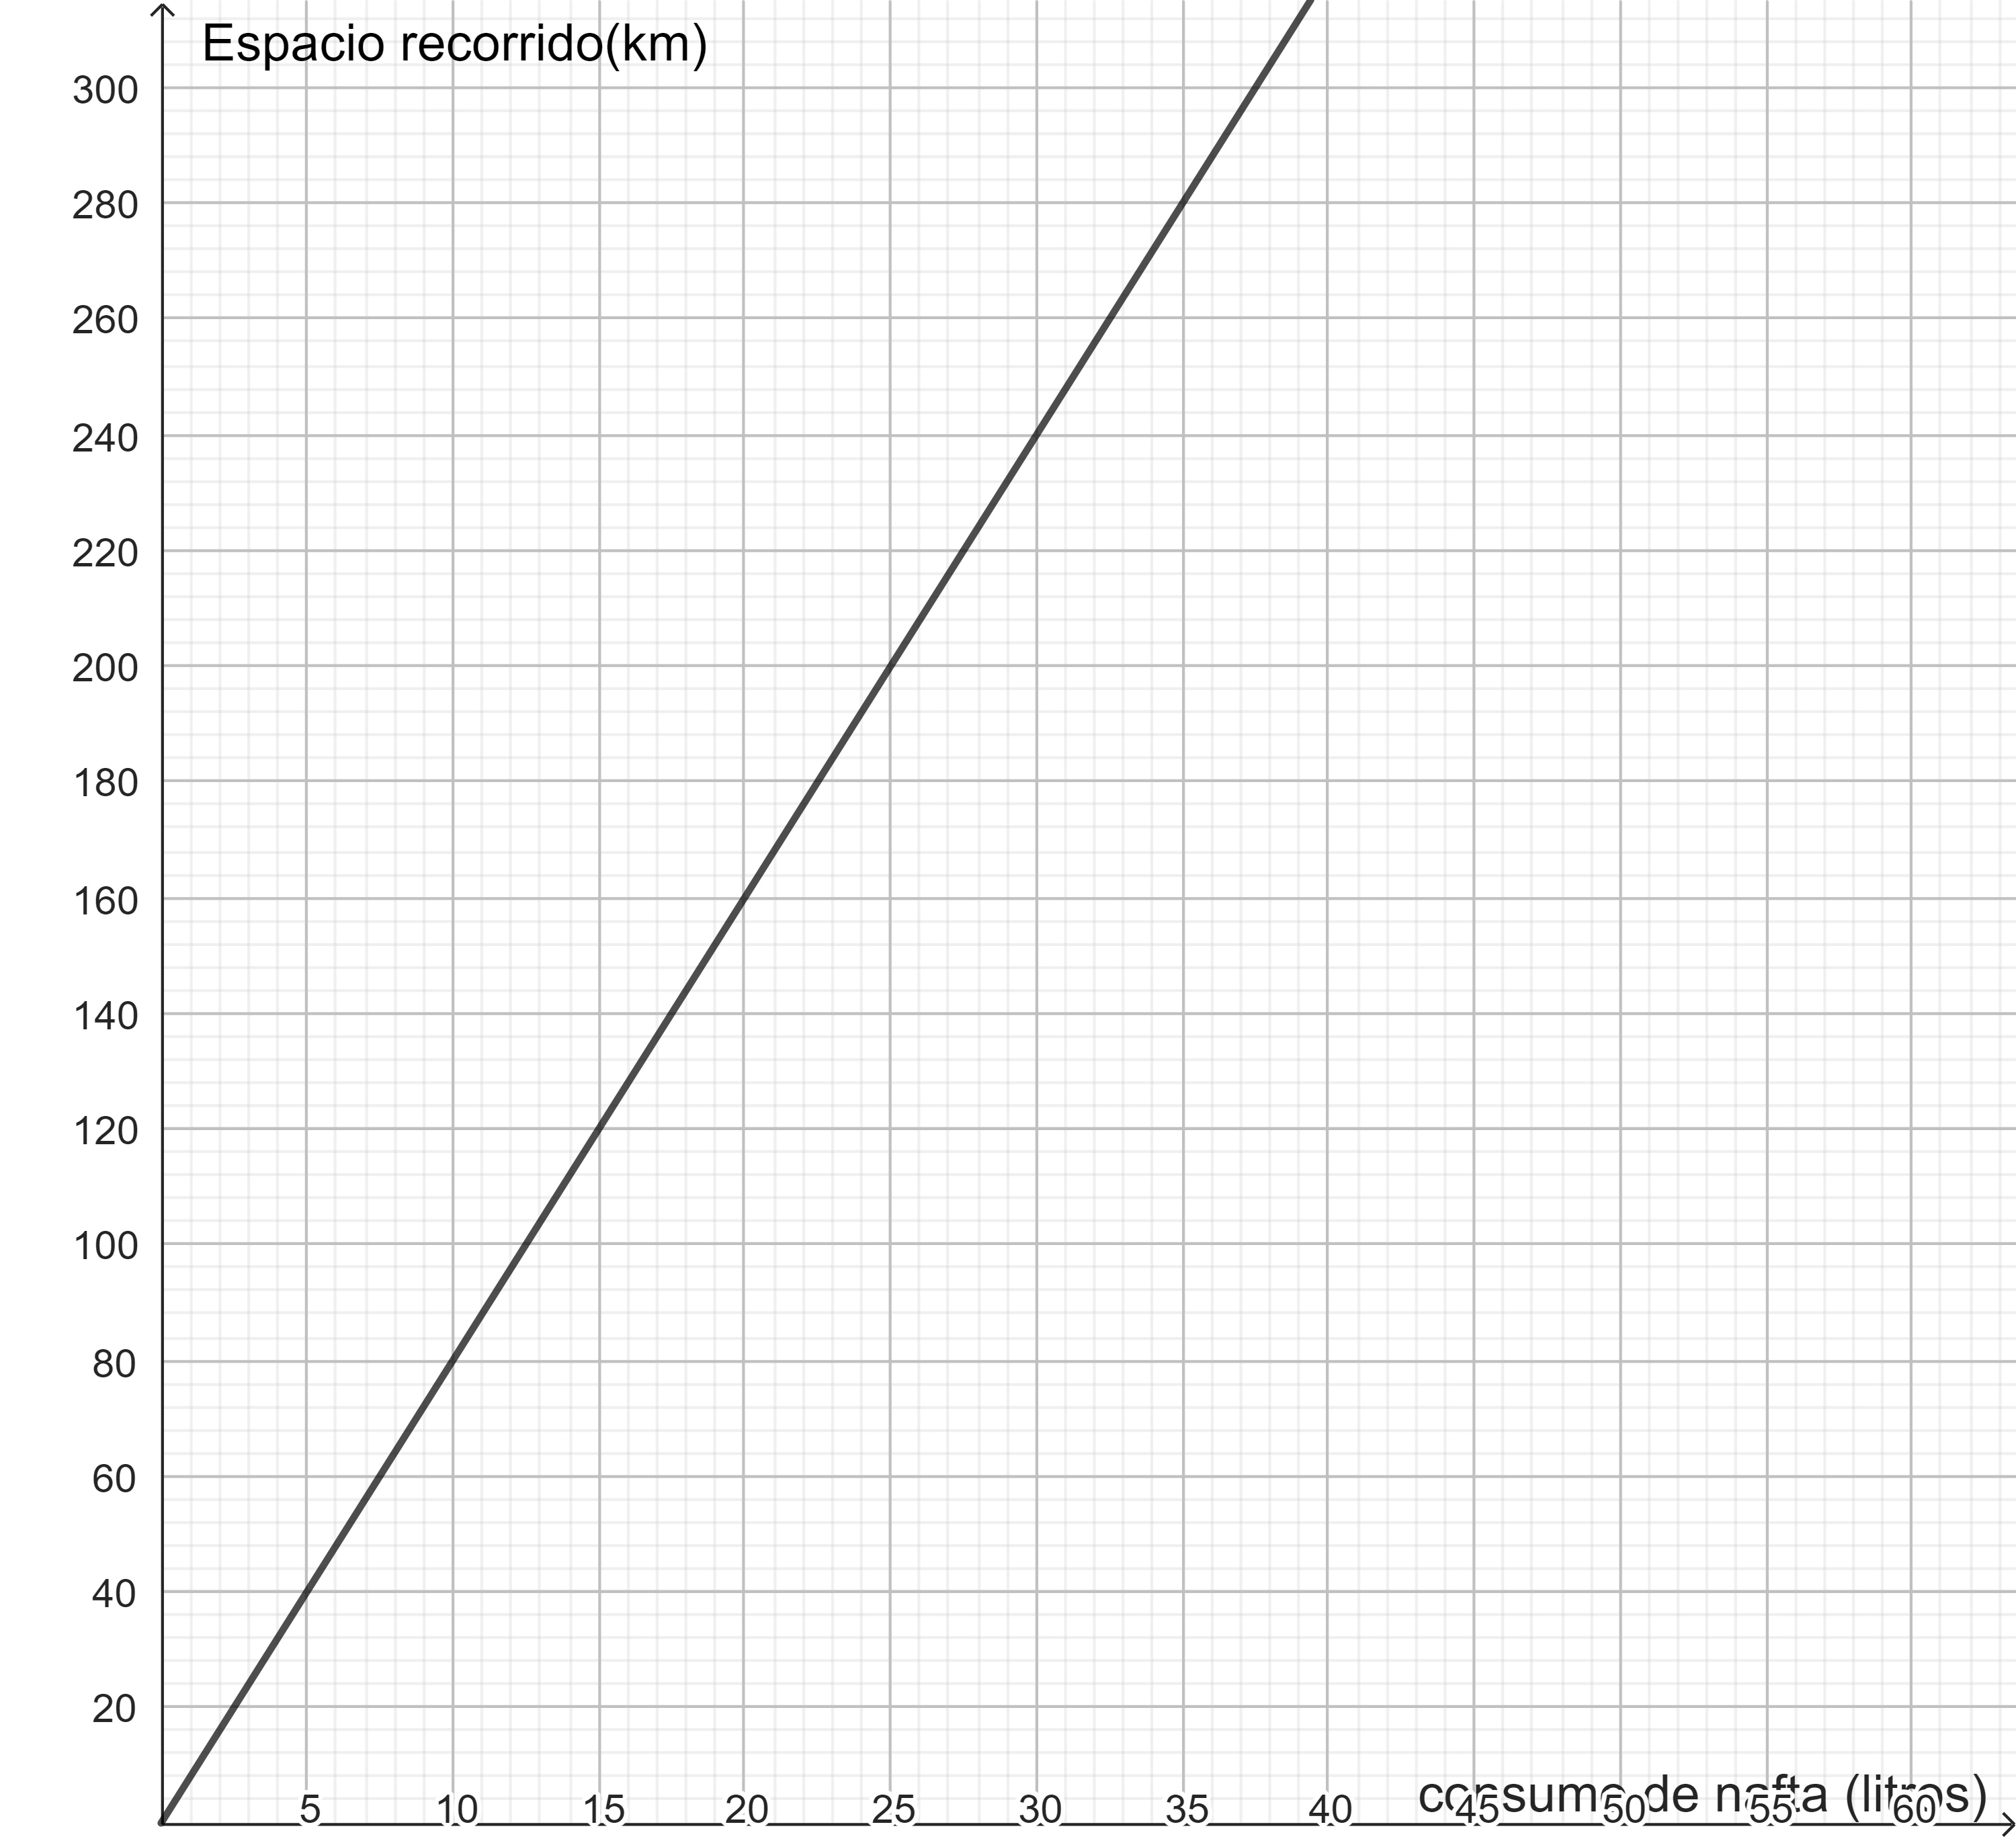
\includegraphics[width=\linewidth]{imagenes/proporcionalidad directa.png}
        \label{fig:proporcionalidad-directa}
      \end{minipage}
      \hfill
      \begin{minipage}[b]{0.3\linewidth}
        \centering
        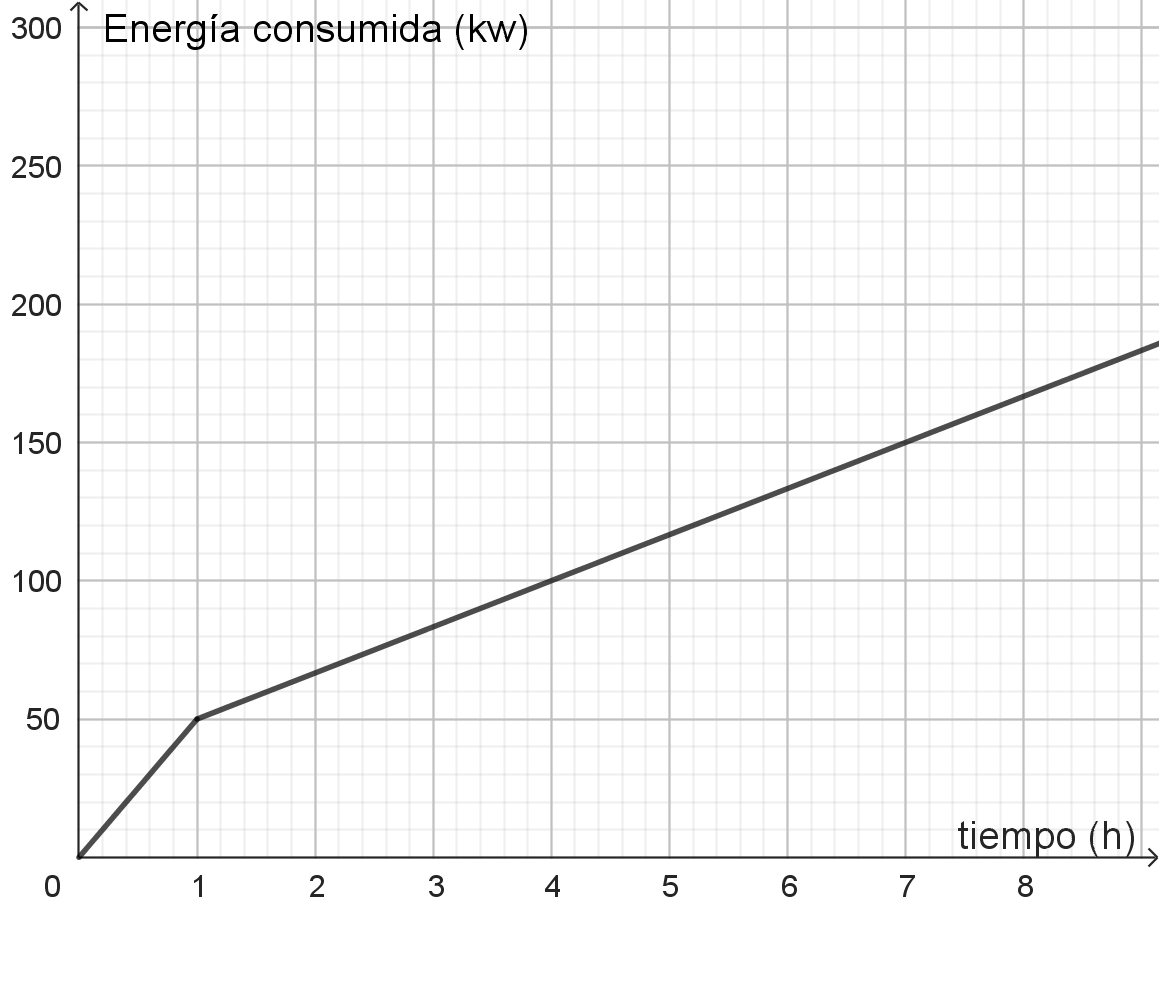
\includegraphics[width=\linewidth]{imagenes/No proporcionalidad directa2.png}
        \label{fig:no-es-proporcionalidad-directa-2}
      \end{minipage}
      \hfill
      \begin{minipage}[b]{0.3\linewidth}
        \centering
        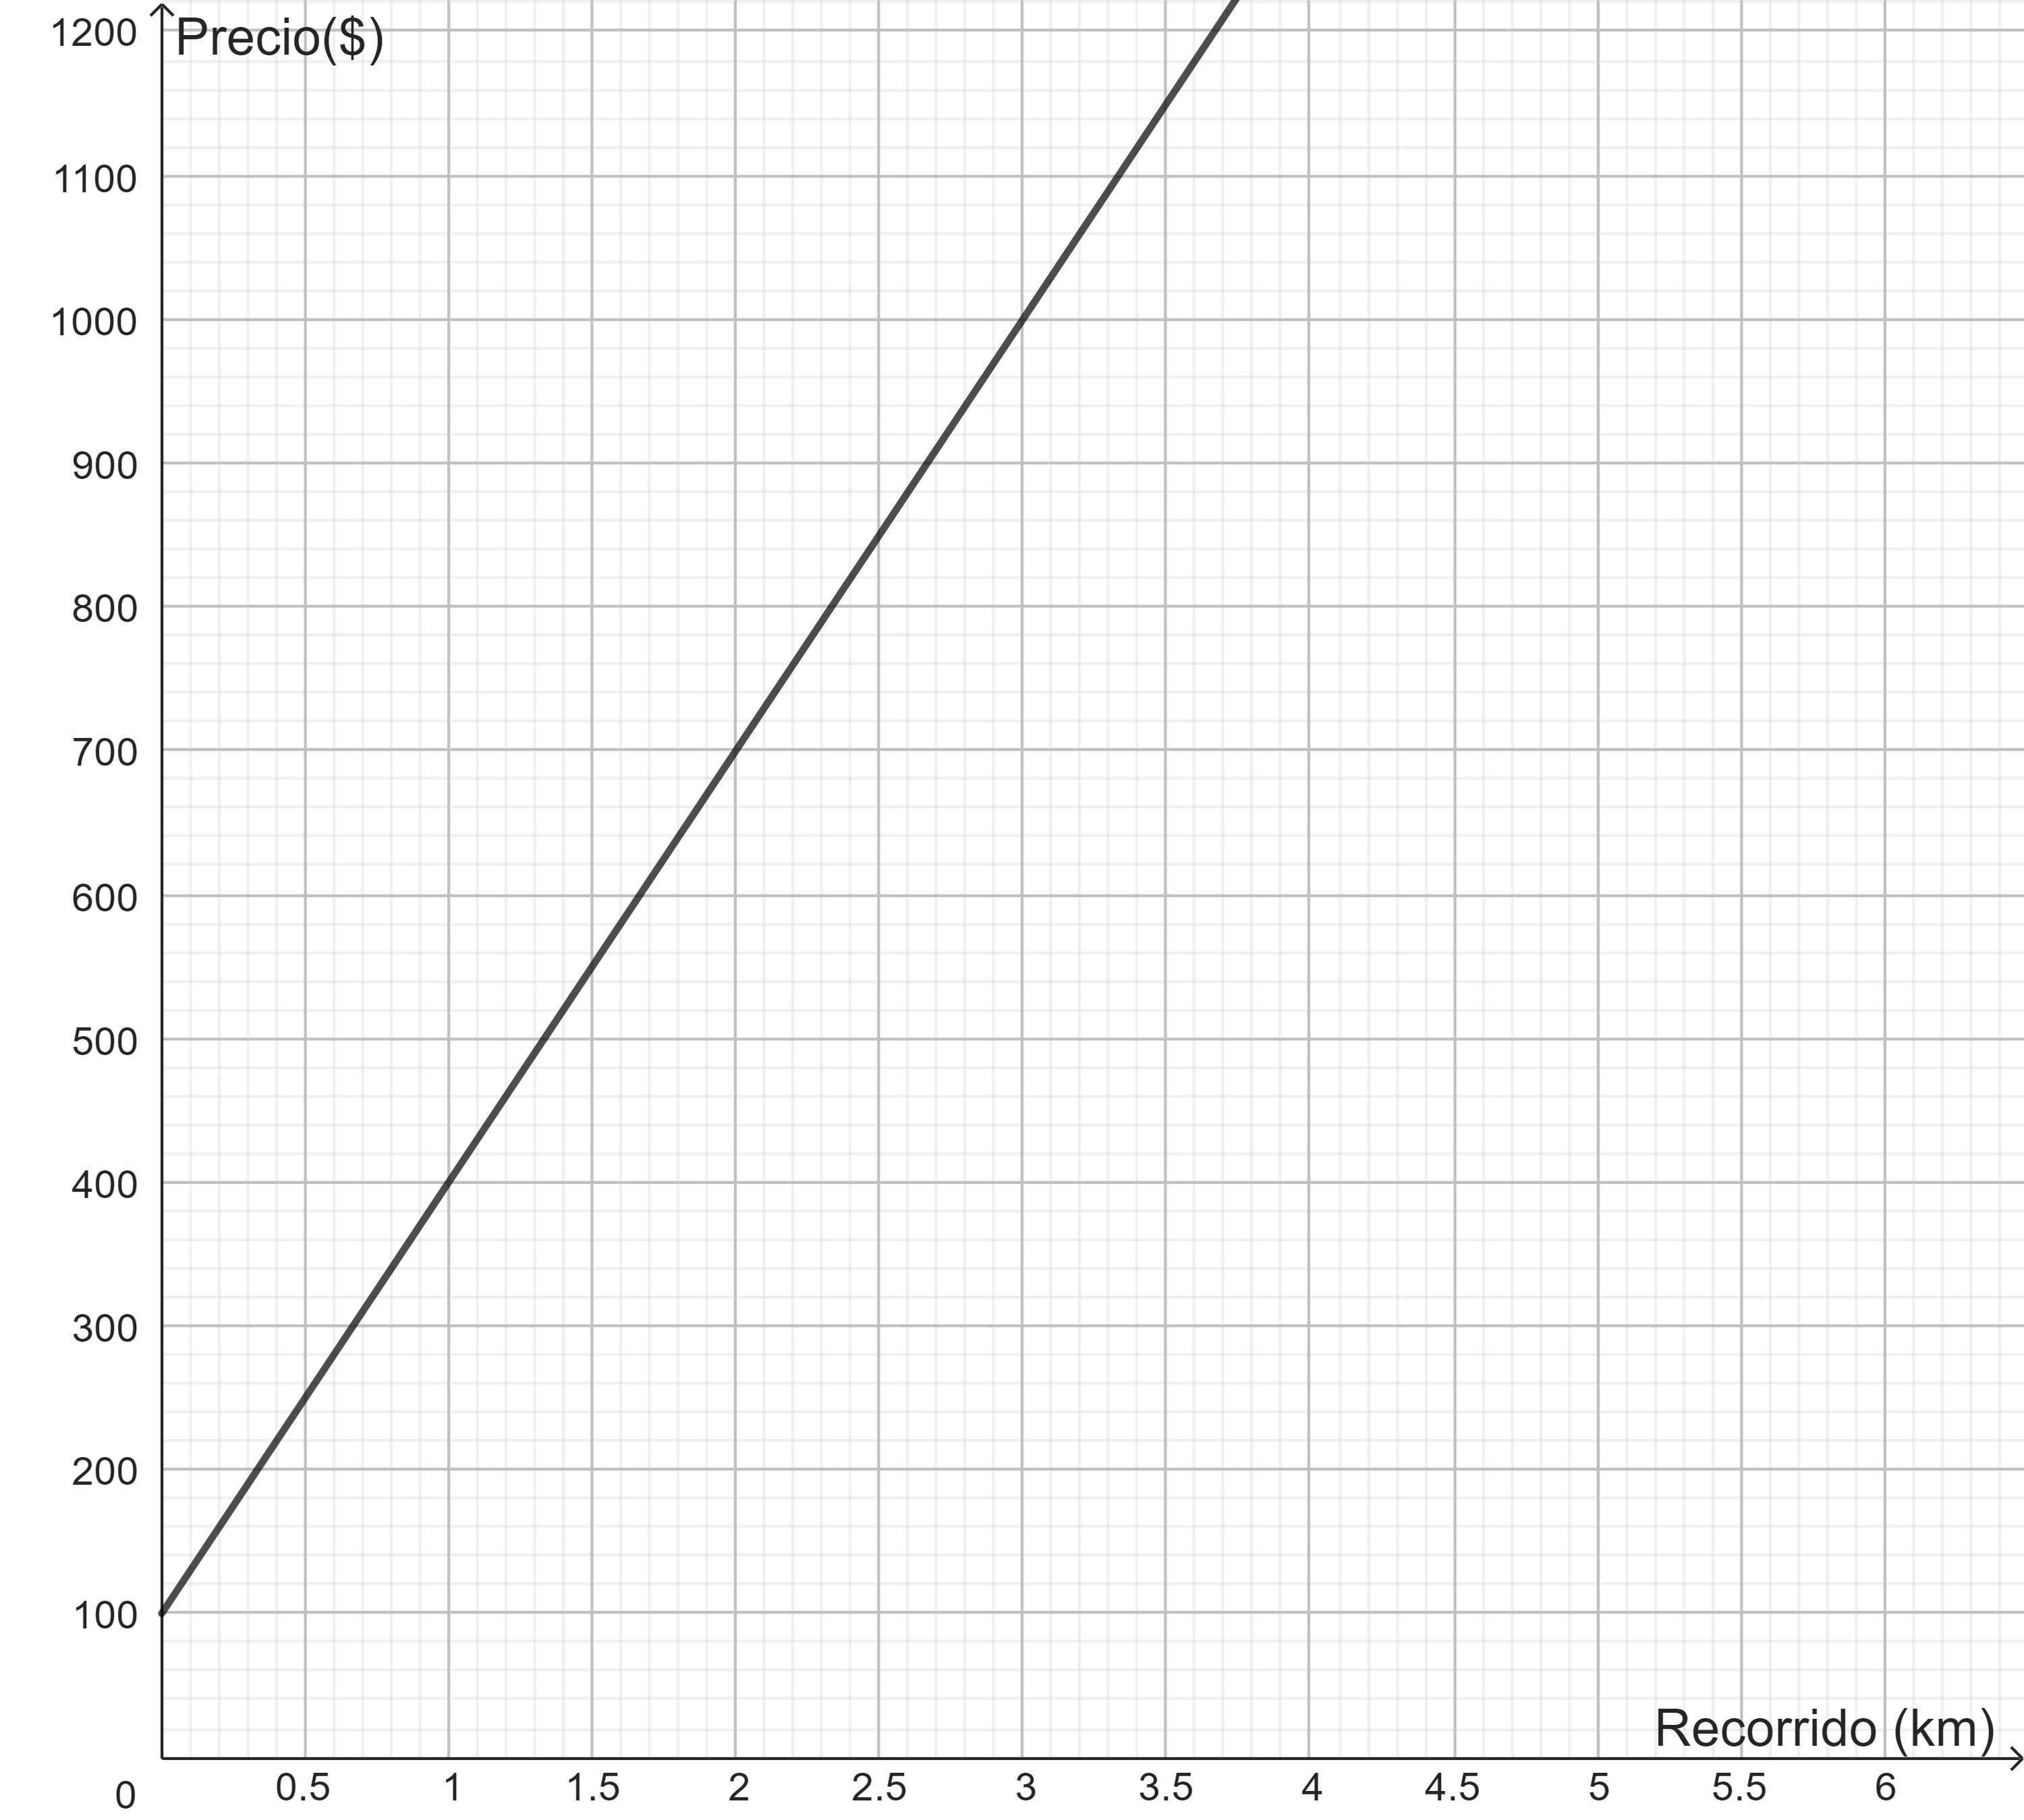
\includegraphics[width=\linewidth]{imagenes/no es proporcionalidad directa.png}
        \label{fig:no-es-proporcionalidad-directa}
      \end{minipage}
    \end{figure}

    ¿Cuál o cuáles corresponden a una proporcionalidad directa? Justifica.
    
    Muestra la/s tabla/s y la expresión algebraica asociada a la relación que corresponda a una proporcionalidad directa.
    
    Se analizará en ellas los contenidos, registros y valor didáctico y posteriormente se realizará la puesta en común.
    
    Se realizará una síntesis final mostrando contenidos, tipo de pensamiento, registros y tipo de actividades sugeridas por nivel para lograr la articulación entre niveles y el desarrollo del pensamiento proporcional.

    
\end{description}

 

\subsection{Evaluación final}

\begin{description}[itemsep=10pt]
    \item[Actividad 1] Deberán responder un cuestionario referido a los contenidos desarrollados en el taller.
    Por ejemplo
    \begin{itemize}[itemsep=10pt]
        \item ¿Cuáles son los tipos de pensamientos proporcionales ? Explique las características de las actividades que desarrollan cada tipo de pensamiento.
        \item ¿En qué consiste “la regla de tres simple” ? ¿cuáles son los obstáculos que genera? Muestre un ejemplo que el estudiante podría resolver aplicando la regla  de tres simple y redacte al menos dos líneas acerca de cómo ud. interactuaría con el estudiante para trabajar sobre ese error.
        \item ¿Se podría calcular porcentajes sin utilizar la regla de tres simple? Explique .
        \item ¿Por qué es importante incluir el uso de Geogebra en la enseñanza de proporcionalidad?

        ...
    \end{itemize}

    \item[Actividad 2]Deberá resolver una actividad de proporcionalidad reconociendo:

    \begin{itemize}[itemsep=10pt]
        \item Contenidos. ( tener en cuenta diseño curricular)
        \item Tipo de pensamiento proporcional.
        \item Significado de proporcionalidad que subyace.
        \item Registro semiótico.
        \item Transformaciones y conversiones de registros.
        \item Año de Primaria o Secundaria al que podría estar dirigido.        
    \end{itemize}

\end{description} 
\section{Bibliografía}

Atela,  M.  A.,  Fernández,  J.  P.,  Vila,  M.  (2019).  Articulación  entre  nivel primario    y    secundario.    Una    experiencia    alrededor    de    la proporcionalidad mediada por TIC. Actas V Jornadas de Enseñanza e Investigación  Educativa  en  el  campo  de  las  Ciencias  Exactas  y Naturales, Fac. de Humanidades y Cs. de la Educación, UNLP.\\

Duval, R.( 2004). Semiosis y Pensamiento Humano. Registros Semióticos y Aprendizajes Intelectuales. Universidad del Valle, Colombia.\\

Godino, J. D., Beltrán-Pellicer, P., Burgos, M., y Giacomone, B. (2017). Significados pragmáticos y configuraciones ontosemióticas en el estudio de la proporcionalidad. En J. M. Contreras, P. Arteaga, G. R. Cañadas, M. M. Gea, B. Giacomone, y M. M. López-Martín (Eds.), Actas del Segundo Congreso International Virtual sobre el Enfoque Ontosemiótico del Conocimiento y la Instrucción Matemáticos (pp. 1-13). 
\href{http://enfoqueontosemiotico.ugr.es/civeos/godino_ beltran.pdf}{http://enfoqueontosemiotico.ugr.es/civeos/godino\_beltran.pdf}\\

\begin{minipage}{1\linewidth}
  \url{http://www.scielo.org.mx/scielo.php?script=sci_arttext&pid=S1665-24362006000200007&lng=es&tlng=es}
\end{minipage}
\\

Mendoza, T. y Block d. (2013) Si 100\% es todo, ¿cuánto es 120\%? Variables didácticas en situaciones de porcentaje. En Broitman C (2013) Matemática en la escuela primaria: saberes y conocimientos de niños y adolescentes. (pag 169-194) , Buenos Aires. Ed. Paidos.\\

Ministerio de Educación, Cultura, Ciencia y Tecnología de la Nación  (2019) .Marco nacional para la mejora del aprendizaje en Matemática. - 1a ed . – Ciudad Autónoma de Buenos Aires.\\

Piaget, J. y Inhelder, B. (1978). Las operaciones intelectuales y su desarrollo. En J. Delval (Ed.),
Lecturas en Psicología del niño, I (pp. 70-119). Madrid: Alianza Editorial.\\

Ruiz, Elena, \& Valdemoros, Marta. (2006). Vínculo entre el pensamiento proporcional cualitativo y cuantitativo: el caso de Paulina. Revista latinoamericana de investigación en matemática educativa, 9(2), 299-324. Recuperado en 03 de junio de 2023, de\\

Van Dooren, W., De Bock, D., Hessels, A., Janssens, D. y Verschaffel, L. (2005). Not everything is proportional: Effects of age and problem type on propensities of overgeneralization. Cognition and Instruction, 23(1), 57-86.


\end{document}
